\documentclass{article}

\usepackage{fontspec}
\usepackage{polyglossia}
\usepackage{notomath}
\setmainfont{GFS Artemisia}
\setsansfont{Source Code Pro}
\setmonofont{Source Code Pro}
\newfontfamily\greekfont[Script=Greek]{GFS Artemisia}
\newfontfamily\greekfontsf[Script=Greek]{GFS Artemisia}
\newfontfamily\greekfonttt[Script=Greek]{Source Code Pro}

%languages
\setdefaultlanguage{greek}
\setotherlanguages{english}


%typing
\usepackage{hyphenat}
\usepackage{float}
\usepackage{color, colortbl}
\usepackage{placeins}

%captions
\usepackage{caption}
\usepackage{subcaption}

%bib
% \usepackage{biblatex}
% \addbibresource{bib.bib}

%gemoetry
\usepackage[a4paper,top=1.2cm,bottom=1.2cm,left=1.2cm,right=1.2cm,marginparwidth=1.5cm]{geometry}

%images
\usepackage{graphicx}
\usepackage{tikz}

%ref
\usepackage[colorlinks=true, allcolors=blue]{hyperref}


\usepackage[export]{adjustbox}

%label
\usepackage{enumitem}
\renewcommand{\labelenumii}{\arabic{enumi}.\arabic{enumii}}
\renewcommand{\labelenumiii}{\arabic{enumi}.\arabic{enumii}.\arabic{enumiii}}
\renewcommand{\labelenumiv}{\arabic{enumi}.\arabic{enumii}.\arabic{enumiii}.\arabic{enumiv}}

%columnnew
\newcolumntype{g}{>{\columncolor{gray}}l}

%colors
\usepackage[dvipsnames]{xcolor}
\definecolor{gray}{gray}{0.9}
\definecolor{blue}{RGB}{82, 138, 174}
\definecolor{green}{RGB}{140, 219, 169}
\definecolor{yellow}{RGB}{253, 221, 92}

% \usepackage{titling}
% \setlength{\droptitle}{-20em}             %allagh glwssas
\hypersetup{
    colorlinks = true,
    linkcolor=black}


\usepackage{autobreak}


%Customize tables
\renewcommand{\arraystretch}{1.2}
% \rowcolors{2}{gray}{white}



\captionsetup[table]{
    format=plain,
    labelfont={small,it,bf}, % Small, italic, and bold label
    textfont={small,it}, % Italic text
    labelsep=colon % Colon separator
}



% Customize the figure caption
\captionsetup[figure]{
    format=plain,
    labelfont={small,it,bf}, % Small, italic, and bold label
    textfont={small,it}, % Italic text
    labelsep=colon % Colon separator
}

\makeatletter
\renewcommand*{\p@table}{\textit{Πίν. }}
\renewcommand*{\p@figure}{\textit{Σχ. }}
\renewcommand*{\p@equation}{\textit{Εξ. }}
\makeatother


\begin{document}

%TITLE
\newcommand{\uni}{ΑΡΙΣΤΟΤΕΛΕΙΟ ΠΑΝΕΠΙΣΤΗΜΙΟ ΘΕΣΣΑΛΟΝΙΚΗΣ}
\newcommand{\faculty}{ΠΟΛΥΤΕΧΝΙΚΗ ΣΧΟΛΗ}
\newcommand{\tmhma}{ΤΜΗΜΑ ΜΗΧΑΝΟΛΟΓΩΝ ΜΗΧΑΝΙΚΩΝ}


\newcommand{\titlos}{Δυναμικά φαινόμενα}
\newcommand{\ypotitlos}{Bonus Εργασία - Ειδικά Κεφάλαια Πεπερασμένων Στοιχείων}


\newcommand{\onomaauthor}{ΒΑΣΙΛΕΙΟΣ ΠΑΠΑΜΙΧΑΗΛ}


\newcommand{\advisor}{Γάκιας Χρήστος}
\newcommand{\mailauthor}{\href{mailto:vasilepi@meng.auth.gr}{vasilepi@meng.auth.gr}}
\newcommand{\aem}{6920}
\newcommand{\hmeromhnia}{\today}



\begin{titlepage}
    \begin{center}
    \raisebox{20mm}{
    \begin{tikzpicture}
        \draw (0,0) -- (6,0);
    \end{tikzpicture}}
\includegraphics[width=4cm]{media/autheng.jpg}\raisebox{20mm}{\begin{tikzpicture}
        \draw (0,0) -- (6,0);
    \end{tikzpicture}}
     \end{center}
    
    \begin{center}
        \large
        \uni\\
        \normalsize
        \faculty\\
        \vspace{1em}
        \tmhma
    \end{center}

    \vspace{2cm}
    \begin{center}
        \Large
        \textbf{\titlos}\\
        \vspace{1em}
        \large
        \textit{\ypotitlos}
    \end{center}
    \begin{center}
        \begin{tikzpicture}
        \draw (0,0) -- (4,0);
    \end{tikzpicture}\\
    \vspace{7em}
    \Large
    \textcolor{BrickRed}{\textbf{\onomaauthor}}\\
    \vspace{3em}
    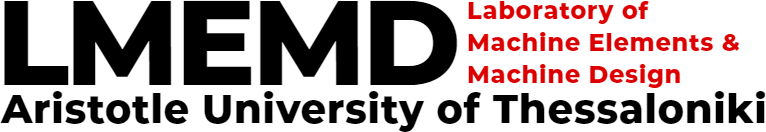
\includegraphics[width=0.3\textwidth]{media/newlogov3-cropped-content.png}
    \end{center}

    \vspace{7em}
    \hspace{4ex}
    \begin{minipage}[t]{0.45\textwidth} 
        \raggedright
        \textbf{Υπεύθυνος}: \advisor\\
        \textbf{Email}: \mailauthor\\
        \textbf{ΑΕΜ}: \aem
    \end{minipage}\\

    \vspace{4cm}
    \begin{center}
        \textit{\hmeromhnia}\\
        \begin{tikzpicture}
            \draw (0,0) -- (15,0);
        \end{tikzpicture}
    \end{center}
    
    
\end{titlepage}

\tableofcontents


\section{Εισαγωγή}
\subsection{Παρουσίαση προβλήματος}
Σκοπός της παρόν εργασίας είναι η επίλυση προβλημάτων επαφών και η εξακρίβωση των αποτελεσμάτων μέσω της θεωρίας επαφών κατά Hertz και της μεθόδου της ποινής. Η εργασία χωρίζεται σε δύο μέρη. 
\par Στο πρώτο μέρος ζητείται η δημιουργία κώδικα που επιλύει απλό πρόβλημα επαφής μεταξύ δύο ράβδων. Τα άκρα των δύο ράβδων είναι πακτωμένα. Οι ράβδοι έχουν αρχικά απόσταση μεταξύ τους. Έπειτα, το ελεύθερο άκρο της μίας ράβδου μετατοπίζεται με τη βοήθεια δύναμης προς την άλλη ράβδο. Μόλις οι δύο ράβδοι βρεθούν σε επαφή επιλύεται το πρόβλημα με τη μέθοδο της ποινής. Ζητούνται τα διαγράμματα δύναμης-μετατόπισης, τα μητρώα στιβαρότητας, τις αναπτυσσόμενες τάσεις και τη δύναμη επαφής.

\begin{figure}[H]
    \centering
    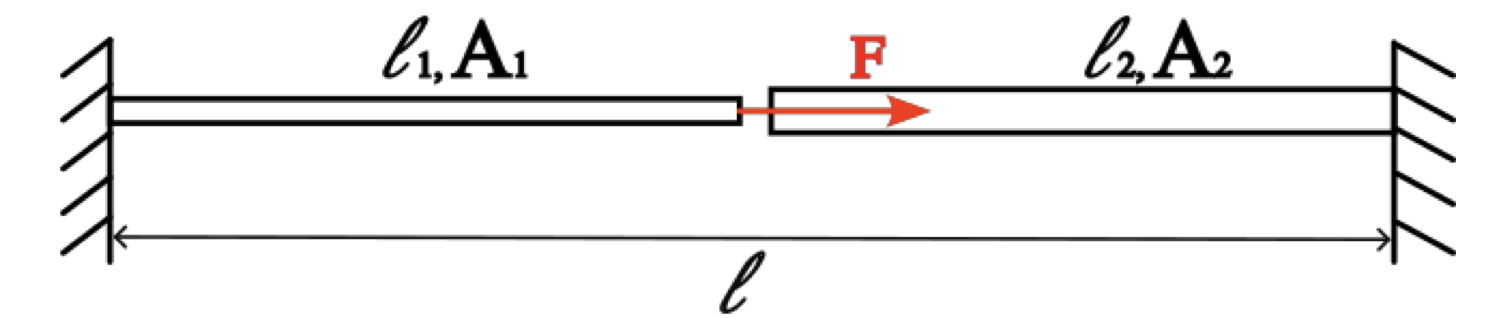
\includegraphics[width=0.6\linewidth]{media/merosA.png}
    \caption{Πρόβλημα πρώτου μέρους.}
    \label{fig:merosA}
\end{figure}

\par Στο δεύτερο μέρος διερευνάται η γραμμική και η σημειακή επαφή μέσω της θεωρίας του Hertz. Ζητείται η δημιουργία δύο μοντέλων για την επίλυση των δύο προβλημάτων. Για τη γραμμική επαφή, δημιουργείται μοντέλο ΠΣ δύο κυλίνδρων σε επαφή. Η δύναμη ασκείται στον έναν κύλινδρο και αναπτύσσονται έτσι οι τάσεις επαφών. Για τη σημειακή επαφή μελετάται η περίπτωση επαφής σφαίρας με επίπεδο. Τα προβλήματα αυτά θα επιλυθούν τόσο με αδρό πλέγμα όσο και με πυκνό. Οι επιλύσεις θα συγκριθούν με τα θεωρητικά αποτελέσματα από τη θεωρία του Hertz. Τα ζητούμενα είναι η αναπτυσσόμενη πίεση και το πλάτος επαφής, οι αναπτυσσόμενες κύριες τάσεις, η σχέση δύναμης-μετατόπισης.
\begin{figure}[H]
    \centering
    \begin{subfigure}{0.49\linewidth}
        \centering
        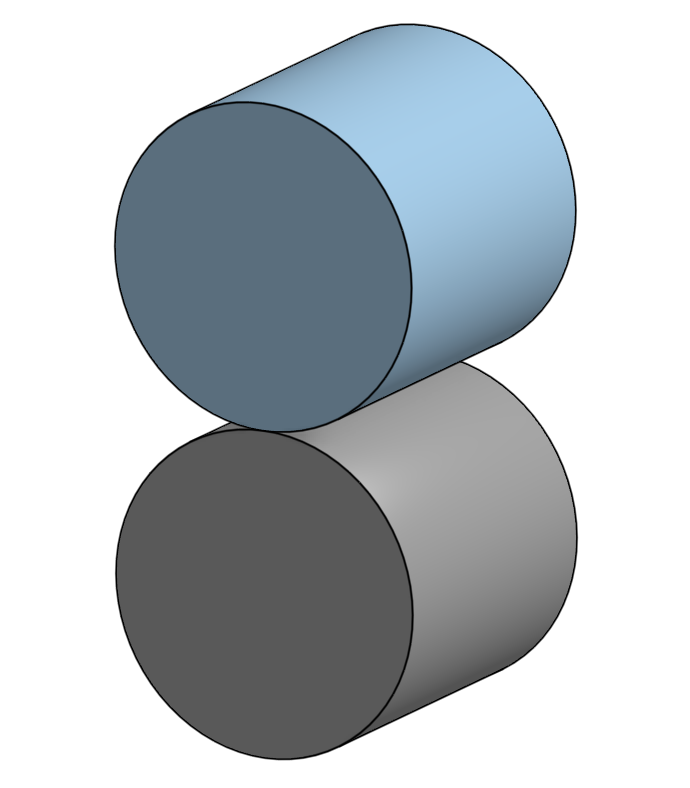
\includegraphics[width=0.6\linewidth]{media/kyl.png}
        \caption{Πρόβλημα γραμμικής επαφής.}
    \end{subfigure}
    \hfill
    \begin{subfigure}{0.49\linewidth}
        \centering
        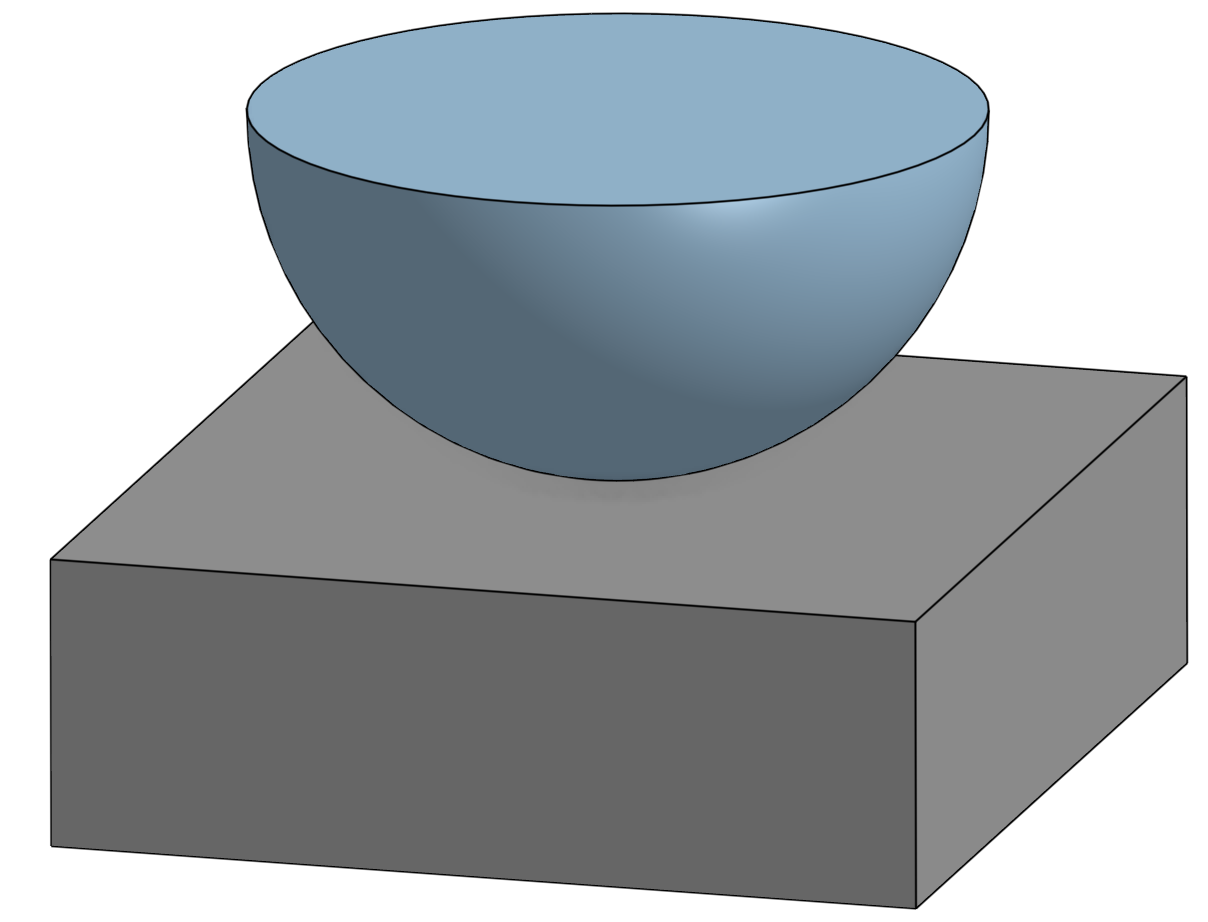
\includegraphics[width=0.6\linewidth]{media/sfaira.png}
        \caption{Πρόβλημα σημειακής επαφής.}
    \end{subfigure}
    \caption{Προβλήματα δεύτερου μέρους.}
    \label{fig:merosB}
\end{figure}



\subsection{Συνοπτική θεωρία}
\subsubsection{Μέθοδος ποινής}
Σύμφωνα με τη μέθοδο της ποινής, αφού τα σώματα έρθουν σε επαφή, ξεκινάει να δρα ένα ελατήριο με πολύ μεγάλη στιβαρότητα στον κόμβο της επαφής. Η σταθερά του ελατηρίου αυτού είναι $\epsilon >> k$. Έτσι, εισάγεται ένα νέο δυναμικό στο ισοζύγιο ενέργειας, αυτό του ελατηρίου με στιβαρότητα $\epsilon$. Πλέον, το πρόβλημα προς ελαχιστοποίηση είναι το:
 \begin{align}
    &\Pi_p = \frac{1}{2}Ku^2 - F u + \frac{1}{2}E g ^2\\
    &\text{s.t.}\;  g\cdot N = 0\\
\end{align}

Με τους πίνακες του συστήματος $K, u, F$ να είναι:
\begin{equation}
    K = \begin{bmatrix}
        k_1 &-k_1 & 0 & 0\\
        -k_1 & k_1 & 0 & 0\\
        0 &0 & k_2 & -k_2\\
        0 &0 & -k_2 & k_2\\
    \end{bmatrix},\; \vec{u} = \begin{pmatrix}
        0\\ u_2 \\ u_3\\ 0
    \end{pmatrix},\; \vec{F} = \begin{pmatrix}
        0\\ F\\ 0\\0
    \end{pmatrix}, \; E = \begin{bmatrix}
        \epsilon & 0 & 0 & 0\\
        0 & \epsilon & 0 & 0\\
         0 & 0 & -\epsilon & 0\\
         0 & 0 & 0 & -\epsilon\\
    \end{bmatrix}, \vec{g} = l - l_1 - l_2 - \vec{u}
\end{equation}

Όπου $N$, η δύναμη επαφής η οποία υπολογίζεται ως:
\begin{equation}
    N = -\epsilon \cdot g
\end{equation}

Τελικά το πρόβλημα καταλήγει στην εξίσωση:
\begin{align}
    K\vec{u} - \vec{F} - E\vec{g} = 0 \\
\end{align}

\begin{figure}[H]
    \centering
    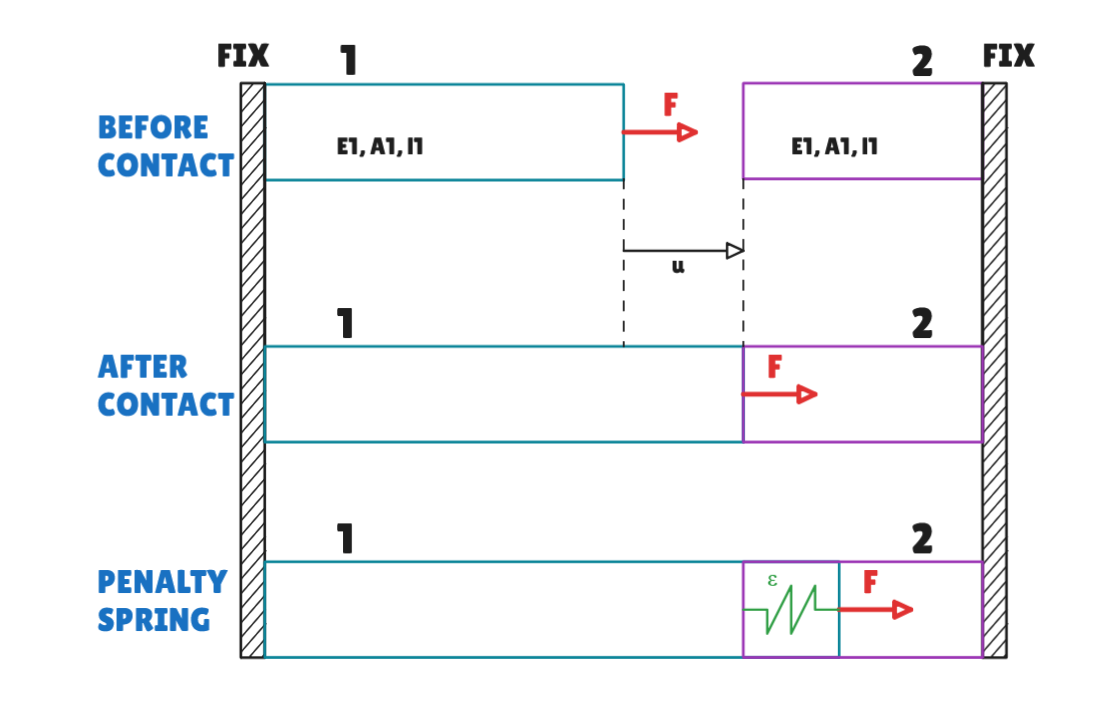
\includegraphics[width=0.6\linewidth]{media/pen.png}
    \caption{Μέθοδος ποινής.}
    \label{fig:pen}
\end{figure}



\subsubsection{Θεωρία Hertz}
Η γραμμική θεωρία του Hertz αναφέρει ότι, κατά την επαφή δημιουργείται ημιπλάτος επαφής που υπολογίζεται ως:
\begin{equation}
    \alpha = \sqrt{\frac{4 F R^*}{\pi E^* l}}
\end{equation}
Με τα ισοδύναμα μεγέθη $Ε^*$, $R^*$, για επαφή δύο κυλίνδρων $R_1, E_1, l$ και $R_2, E_2, l$ να υπολογίζονται ως:
\begin{align}
    \frac{1}{E^*} & = \frac{1-\nu_1^2}{E_1} + \frac{1-\nu_2^2}{E_2} \\
    \frac{1}{R^*} &= \frac{1}{R_1} + \frac{1}{R_2} 
\end{align}

Η πίεση επαφής κατά την διεύθυνση της επαφής δίνεται ως:
\begin{equation}
    p = \frac{2F}{\pi \alpha l} \sqrt{1 - \bigg(\frac{x}{\alpha}\bigg)^2} = p_0\sqrt{1 - \bigg(\frac{x}{\alpha}\bigg)^2}
\end{equation}


Η σχέση δύναμης μετατόπισης είναι γραμμική και δίνεται ως:
\begin{equation}
    F = \frac{\pi}{4}E^* l u
\end{equation}

Τέλος, οι κύριες τάσεις συναρτήσει του βάθους στον κύλινδρο δίνονται ως:
\begin{align}
    \sigma_x &= -2\nu p_0 \bigg(\sqrt{1 + \bigg(\frac{z}{\alpha}\bigg)^2} - \bigg|\frac{z}{\alpha}\bigg|\bigg)\\

    \sigma_y &= - p_0 \Bigg(\frac{1+2\frac{z^2}{\alpha^2}}{\sqrt{1 + \bigg(\frac{z}{\alpha}\bigg)^2}} - 2\bigg|\frac{z}{\alpha}\bigg|\Bigg)\\

    \sigma_z &= -\frac{p_0}{\sqrt{1 + \bigg(\frac{z}{\alpha}\bigg)^2}}
\end{align}



Αντίστοιχα, η θεωρία του Hertz για σημειακή επαφή, δηλαδή επαφή δύο σφαιρών,  αναφέρει ότι το πλάτος επαφής είναι:

\begin{equation}
    \alpha = \sqrt[3]{\frac{3 F R^*}{4 E^*}}
\end{equation}
Με τα ισοδύναμα μεγέθη $E^*$, $R^*$ να δίνονται με τον ίδιο τρόπο όπως στην επαφή των κυλίνδρων. Η πίεση επαφής κατά την ακτινική διεύθυνση δίνεται ως:
\begin{equation}
    p = \frac{3F}{2\pi \alpha^2} \sqrt{1 - \bigg(\frac{r}{\alpha}\bigg)^2} = p_0\sqrt{1 - \bigg(\frac{r}{\alpha}\bigg)^2}
\end{equation}

Στην περίπτωση επαφής σφαίρας δαπέδου απλώς ορίζεται ότι $R_2 = \inf$. Η σχέση δύναμης μετατόπισης δεν είναι γραμμική αυτή τη φορά και δίνεται ως:
\begin{equation}
    F = \frac{4}{3}E^* \sqrt{R^*} u^{3/2}
\end{equation}

Τέλος, οι κύριες τάσεις συναρτήσει του βάθους δίνονται ως:
\begin{align}
    \sigma_{x,y} &= - p_0 \bigg( \bigg(1-\bigg|\frac{z}{\alpha}\bigg| atan\bigg(\frac{1}{|z/\alpha|}\bigg)\bigg)(1+\nu)  - \frac{1}{2 (1 + \bigg(\frac{z}{\alpha}\bigg)^2)} \bigg)\\

    \sigma_z &= -\frac{p_0}{1 + \bigg(\frac{z}{\alpha}\bigg)^2}
\end{align}

\section{Μοντελοποίηση}

\subsection{Μέρος Α'}
Για το πρώτο μέρος της εργασίας, η μοντελοποίηση αφορά την επίλυση του συστήματος των εξισώσεν που παρουσιάστηκαν παραπάνω. Ορίζοντας τους κόμβους και τα στοιχεία του συστήματος, το πρόβλημα έγκειται στην επίλυση του απλού συστήματος $4\times 4$. Ωστόσο, μιας και οι κόμβοι 1 και 4 είναι πακτωμένοι, διαγράφοντας τις αντίστοιχες γραμμές και στήλες, το πρόβλημα καταλήγει στο σύστημα $2\times 2$ εξισώσεων:
\begin{align}
    k_1 u_2 - F - \epsilon (l-l_1-l_2-u_2) =& 0\\
    k_2 u_3 + \epsilon (l - l_1 -l_2 - u_3) =& 0
\end{align}

\begin{figure}[H]
    \centering
    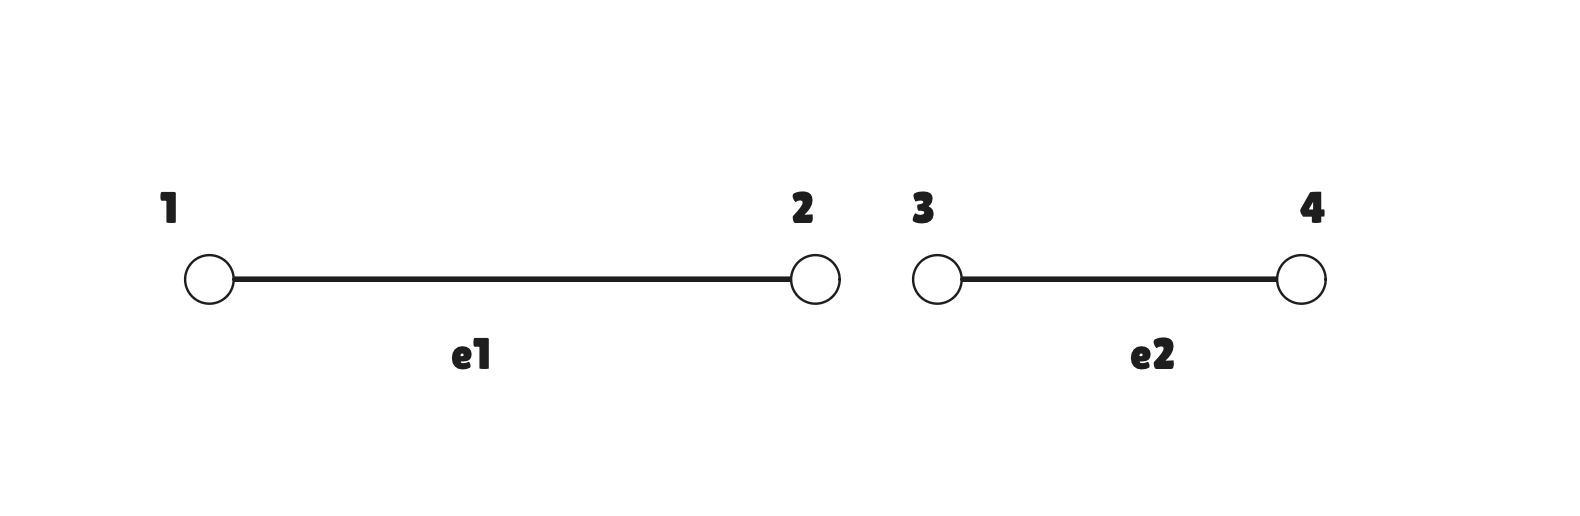
\includegraphics[width=0.6\linewidth]{media/nodes.png}
    \caption{Μοντελοποίηση προβλήματος πρώτου μέρους.}
    \label{fig:nodes}
\end{figure}

Προφανώς, κατά την επαφή θα ισχύει ότι οι κόμβοι 2 και 3 κινούνται μαζί. Έτσι, αναμένεται οι μετατοπίσεις τους να έχουν αντίθετη φορά και έως ότου αρχίσει η επαφή ο κόμβος 2 να έχει μηδενική μετατόπιση.

\subsection{Μέρος Β'}
Στο δεύτερο μέρος, ζητούνται μοντέλα επαφών ΠΣ. Ζητείται η μοντελοποίηση τόσο με αδρό πλέγμα όσο και με πυκνό. Για το αδρό πλέγμα η προϋπόθεση είναι ότι ο μέγιστος αριθμός κόμβων δεν πρέπει να ξεπερνάει το όριο της φοιτητικής αδείας. Επομένως, τα μοντέλα των κυλίνδρων δημιουργούνται μισά και αντίστοιχα της σφαίρας επίσης μισό. Το δάπεδο στο οποίο ακουμπάει η σφαίρα, με άπειρη ακτίνα, πρέπει να έχει πάχος παρόμοιο με αυτό της σφάιρας.  
\par Όσο αναφορά τις παραμέτρους επίλυσης, γεωμετρικά τα μοντέλα δεν ακουμπάνε. Έτσι, ορίζεται η παράμετρος \texttt{ADJUST} στη καρτέλα της επαφής, ώστε να μετακινηθούν τα σώματα το ένα μέσα στο άλλο για να ξεκινήσει η επίλυση της επαφής. Οι οριακές συνθήκες των δύο προβλημάτων φαίνονται παρακάτω.

\begin{table}[H]
    \centering
    \rowcolors{2}{gray}{white}
    \begin{tabular}{|c|c|}
        \hline
        \rowcolor{Dandelion}
        \multicolumn{2}{|c|}{Linear}\\ \hline
        Επιφάνεια εφαρμογής δύναμης & Περιορισμός στο επίπεδο της\\
        \hline
        Eλεύθερη επιφάνεια μη φορτισμένου κυλίνδρου & Περιορισμός σε όλους τους μεταφορικούς β.ε.\\
        \hline
        Άξονες συμμετρίας κυλίνδρων στη μία πλευρά & Περιορισμός στο β.ε. κατά την εγκάρσια στον άξονα διεύθυνση\\ \hline
        \rowcolor{yellow}
        \multicolumn{2}{|c|}{Point}\\ \hline
        Επιφάνεια εφαρμογής δύναμης & Περιορισμός στο επίπεδο της\\
        \hline
        Επίπεδη ελεύθερη επιφάνεια δαπέδου & Περιορισμός σε όλους τους μεταφορικούς β.ε.\\
        \hline
    \end{tabular}
    \caption{Οριακές συνθήκες προβλημάτων επαφής.}
    \label{tab:bcs}
\end{table}

Παρακάτω φαίνονται τα μοντέλα ΠΣ των προβλημάτων καθώς και οι περιοχές πύκνωσης με πλάτος λίγο περισσότερο από το θεωρητικά αναμενόμενο πλάτος επαφής.

\begin{figure}[H]
    \centering
    \begin{subfigure}{0.49\linewidth}
        \centering
        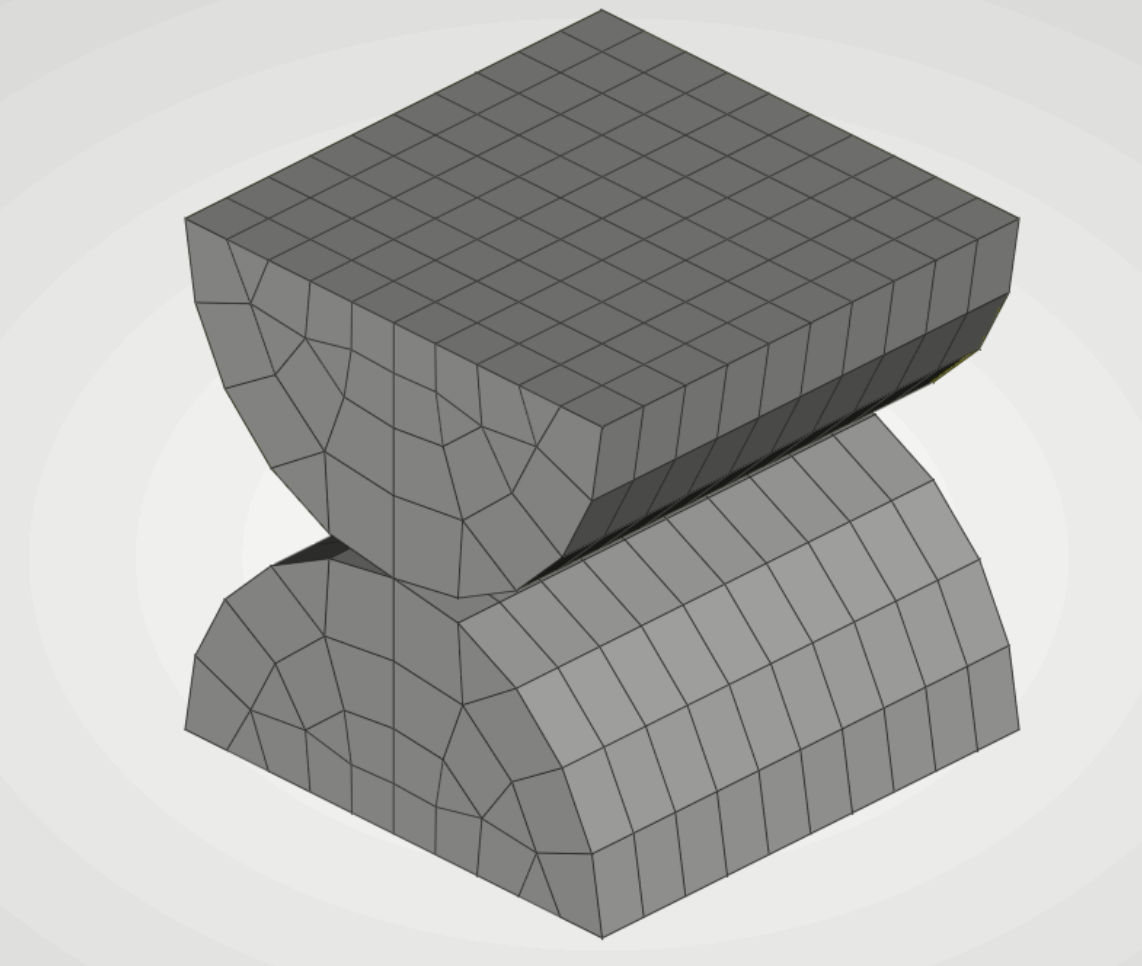
\includegraphics[width=0.7\linewidth]{media/lcoarse.png}
        \caption{Μοντέλο γραμμικής επαφής.}
    \end{subfigure}
    \hfill
    \begin{subfigure}{0.49\linewidth}
        \centering
        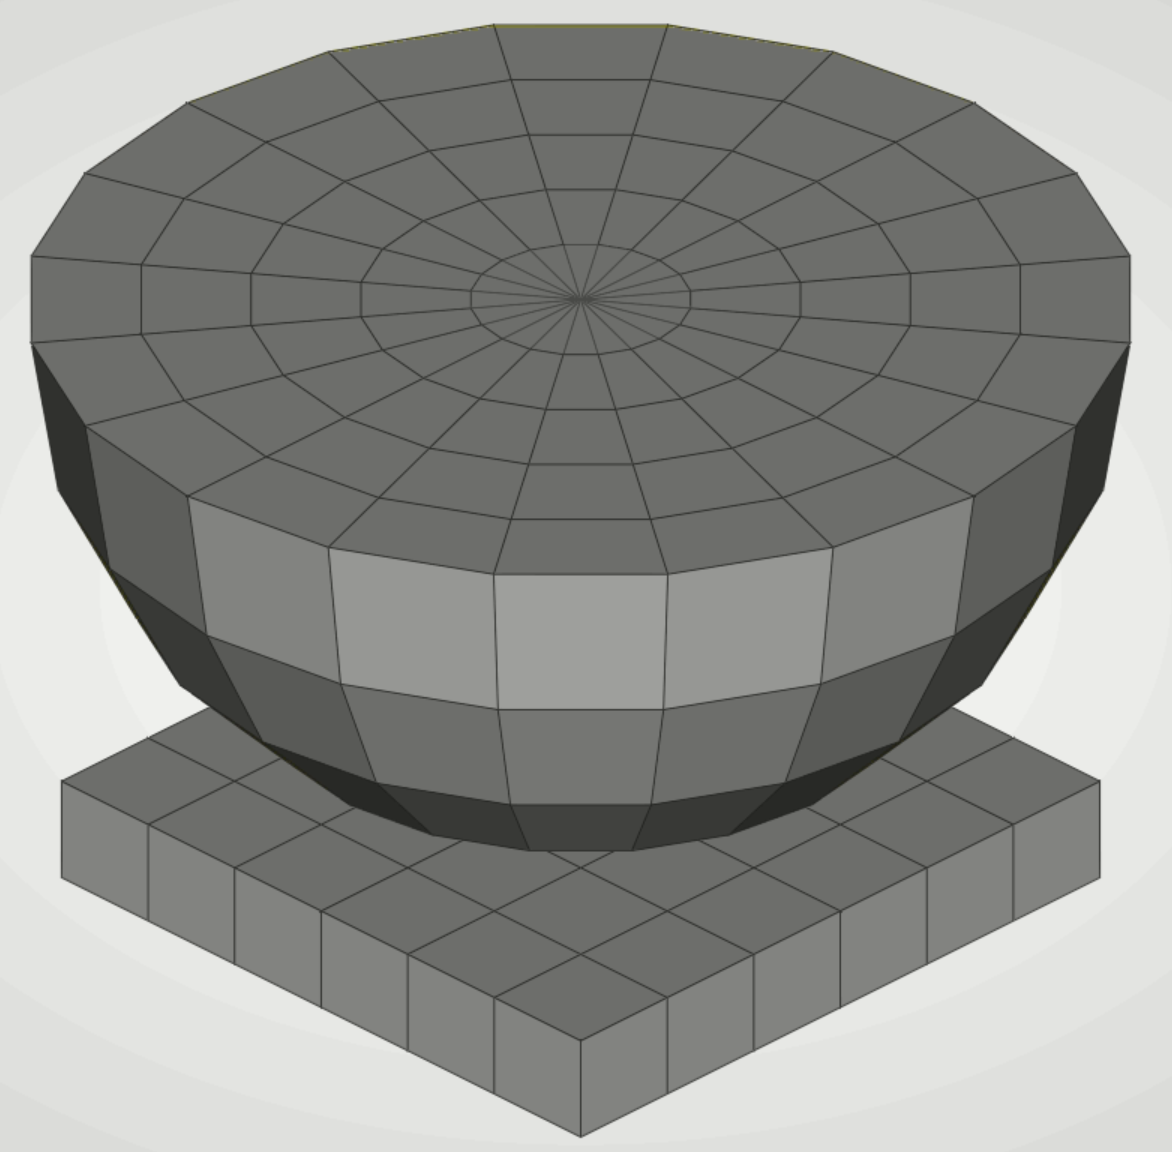
\includegraphics[width=0.6\linewidth]{media/pcoarse.png}
        \caption{Μοντέλο σημειακής επαφής.}
    \end{subfigure}
    \caption{Μοντέλα πεπερασμένων στοιχείων με αδρό πλέγμα.}
    \label{fig:mod}
\end{figure}

\begin{figure}[H]
    \centering
    \begin{subfigure}{0.49\linewidth}
        \centering
        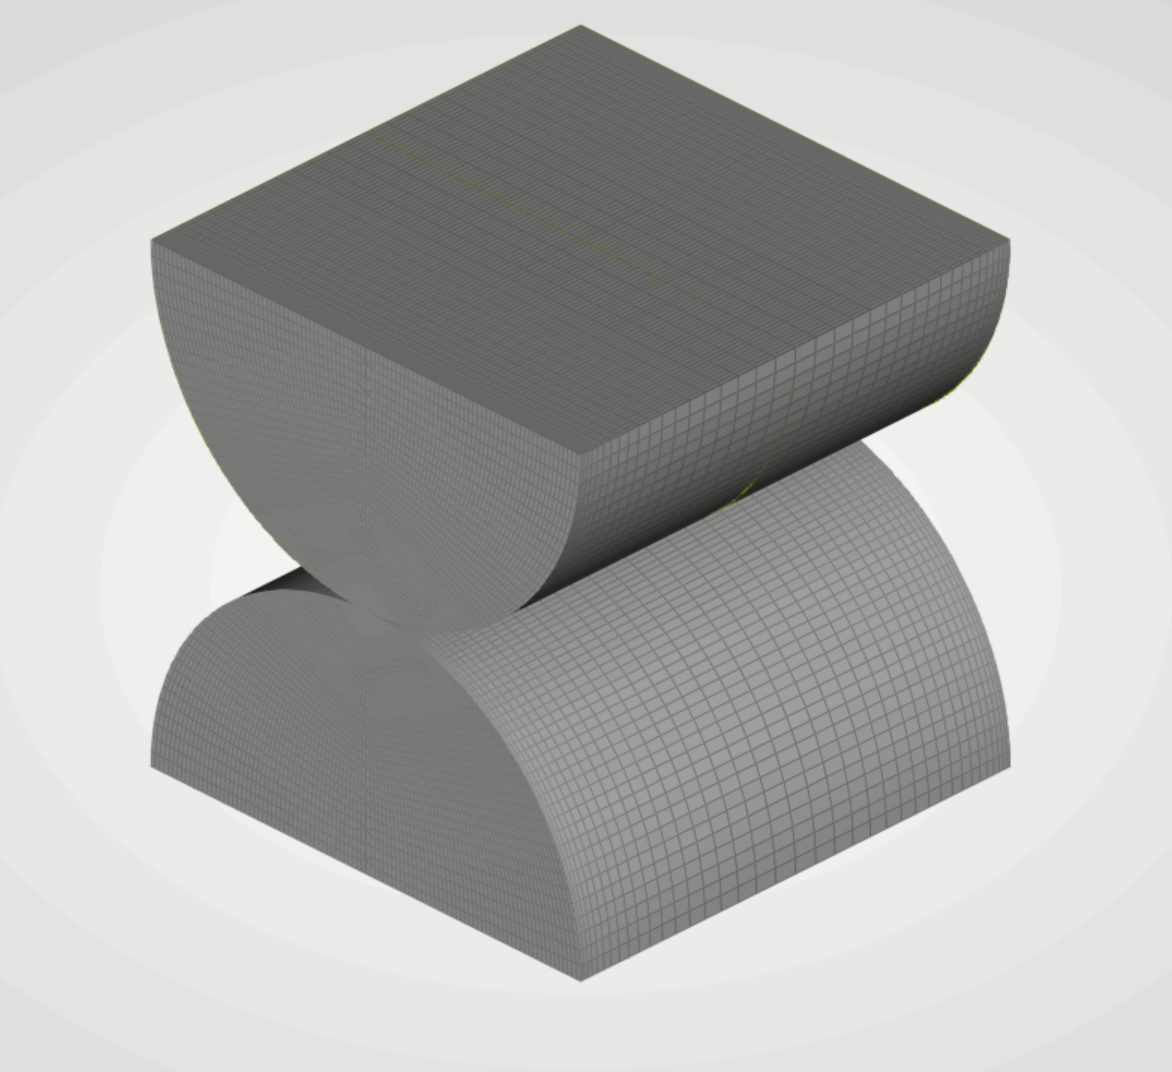
\includegraphics[width=0.7\linewidth]{media/lfine.png}
        \caption{Μοντέλο γραμμικής επαφής.}
    \end{subfigure}
    \hfill
    \begin{subfigure}{0.49\linewidth}
        \centering
        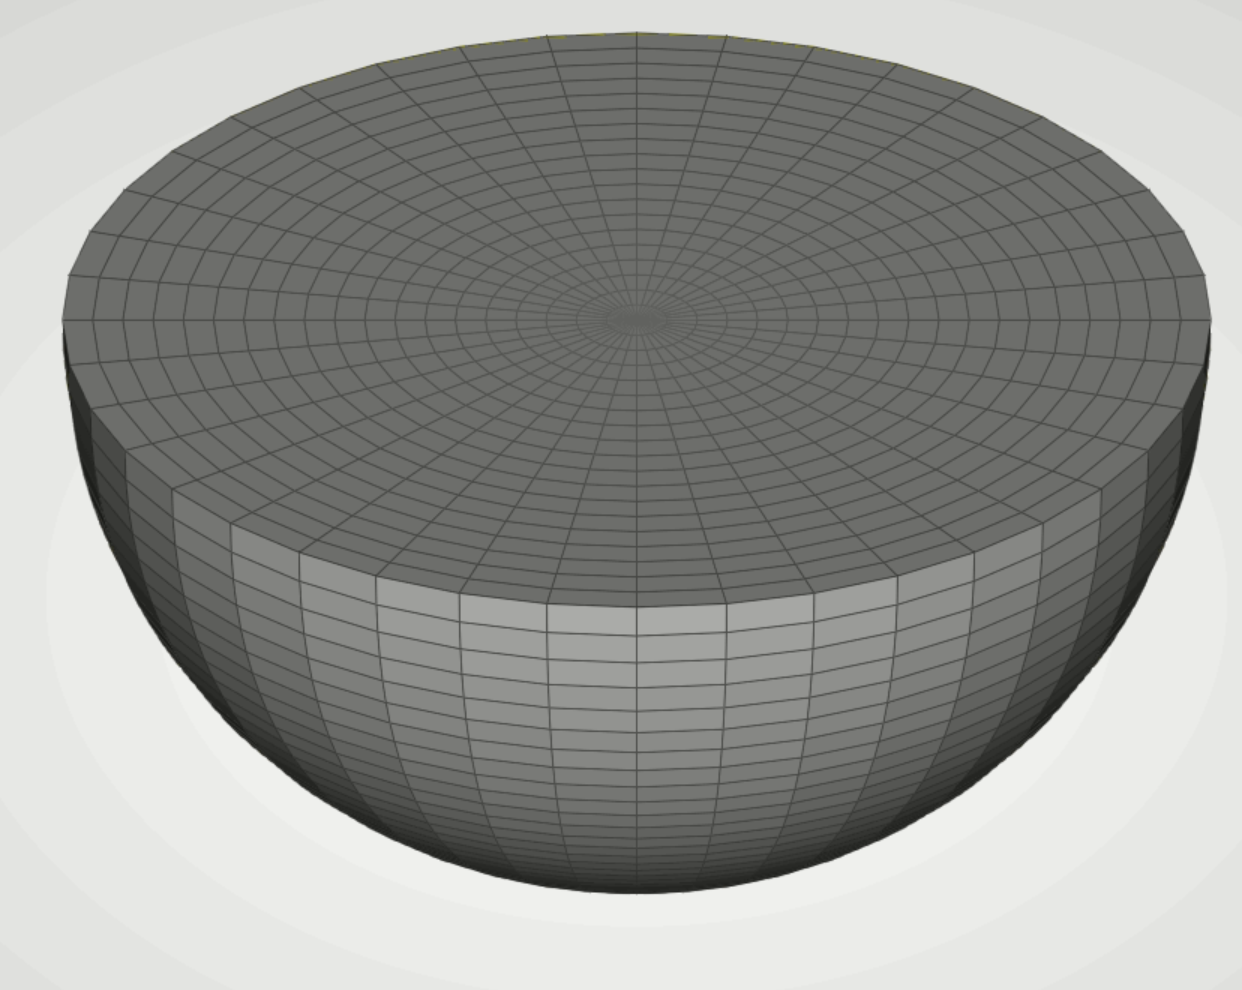
\includegraphics[width=0.8\linewidth]{media/pfine.png}
        \caption{Μοντέλο σημειακής επαφής.}
    \end{subfigure}
    \caption{Μοντέλα πεπερασμένων στοιχείων με πυκνό πλέγμα.}
    \label{fig:mod2}
\end{figure}

\begin{figure}[H]
    \centering
    \begin{subfigure}{0.49\linewidth}
        \centering
        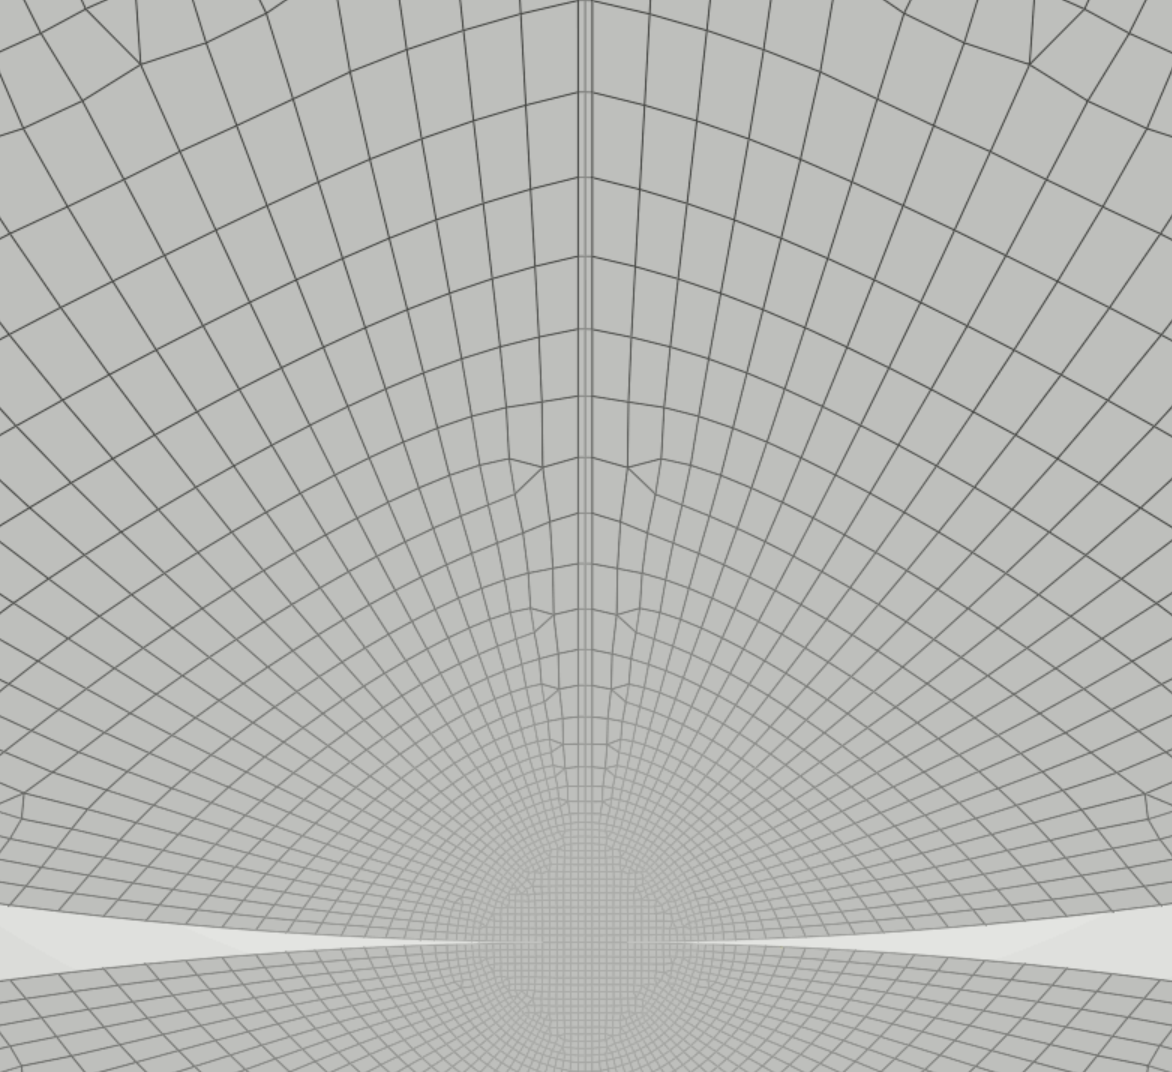
\includegraphics[width=0.6\linewidth]{media/lfine2.png}
        \caption{Μοντέλο γραμμικής επαφής.}
    \end{subfigure}
    \hfill
    \begin{subfigure}{0.49\linewidth}
        \centering
        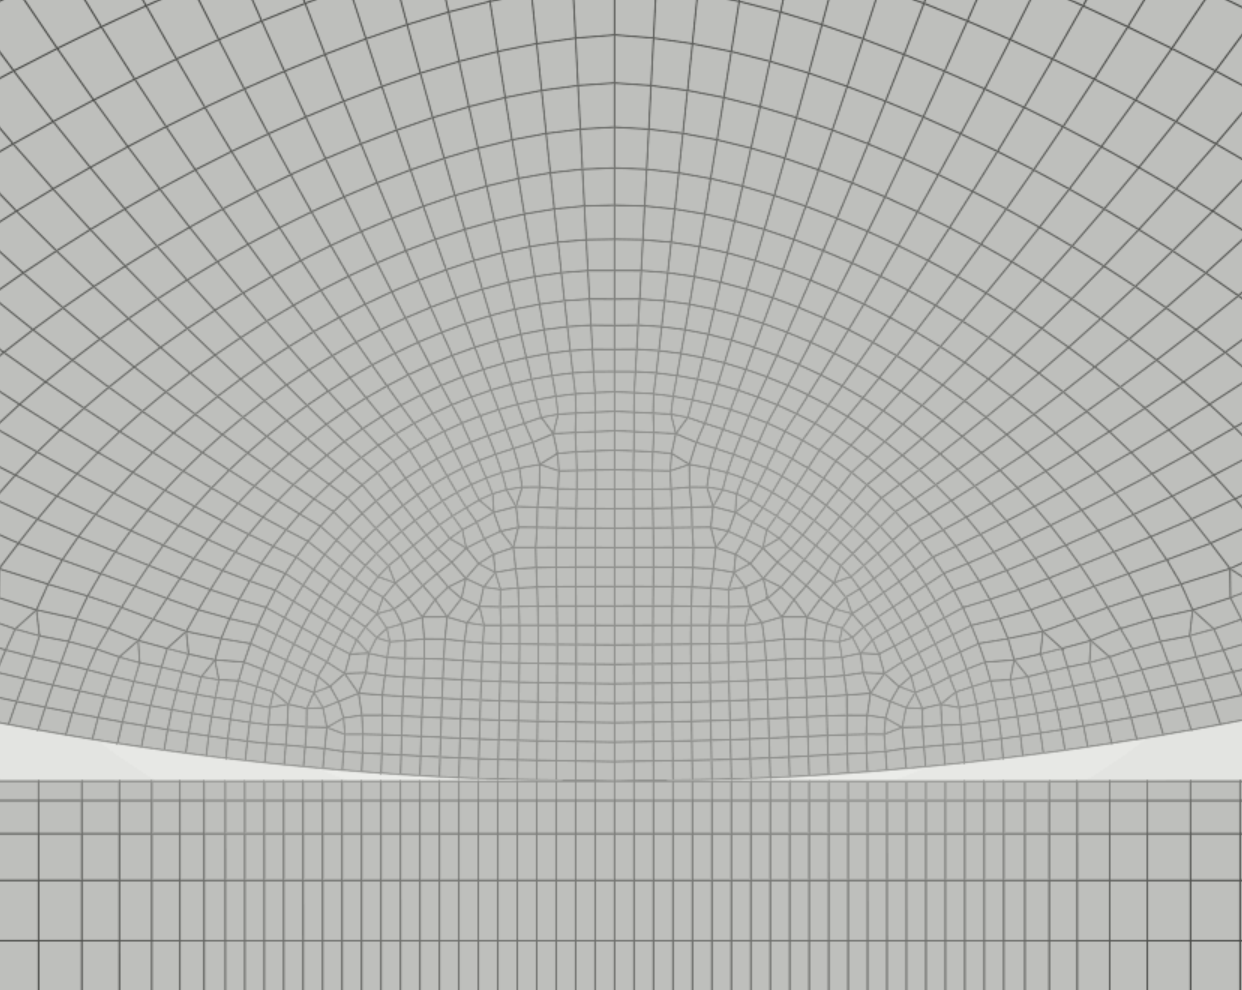
\includegraphics[width=0.7\linewidth]{media/pfine2.png}
        \caption{Μοντέλο σημειακής επαφής.}
    \end{subfigure}
    \caption{Πύκνωση πλέγματος στο σημείο επαφής.}
    \label{fig:mod3}
\end{figure}


\section{Αποτελέσματα Και Συζήτηση}
\subsection{Μέρος Α'}
Από την επίλυση του προγράμματος για το πρώτο μέρος προκύπτουν η δύναμη αντίδρασης στην επαφή, οι μετατοπίσεις των δύο ράβδων και οι τάσεις που προκύπτουν στη κάθε ράβδο. Στον \ref{tab:ded} φαίνονται τα δεδομένα της επίλυσης και στον \ref{tab:apot} τα αποτελέσματα του πρώτου μέρους.
\begin{table}[H]
    \centering
    \rowcolors{2}{gray}{white}
    \begin{tabular}{|c|c|}
        \hline
        \rowcolor{Dandelion}
        Δεδομένο & Τιμή\\ \hline
        $F$ & $8000\; N$\\ \hline
        $l$ & $1505\; mm$\\ \hline
        $l_1$ & $500\; mm$\\ \hline
        $l_2$ & $1000\; mm$\\ \hline
        $A_1$ & $1.8\; mm^2$\\ \hline
        $A_2$ & $3.1\; mm^2$\\ \hline
        $\epsilon$ & 1E10 \\ \hline
    \end{tabular}
    \caption{Δεδομένα προβλήματος πρώτου μέρους.}
    \label{tab:ded}
\end{table}

\begin{table}[H]
    \centering
    \rowcolors{2}{gray}{white}
    \begin{tabular}{|c|c|}
        \hline
        \rowcolor{yellow}
        Αποτέλεσμα & Τιμή\\ \hline
        $N$ & $1952\; N$\\ \hline
        $u_2$ & $7.999\; mm$\\ \hline
        $u_3$ & $-2.999\; mm$\\ \hline
        $\sigma_1$ & $3359\; MPa$\\ \hline
        $\sigma_2$ & $-629\; MPa$\\ \hline
    \end{tabular}
    \caption{Αποτελέσματα προβλήματος πρώτου μέρους.}
    \label{tab:apot}
\end{table}

Να σημειωθεί, ότι η τιμή για τη σταθερά ποινής δοκιμάστηκε. Όπως αναμενόταν πολύ μεγάλες τιμές της κάουν το πρόβλημα ασταθές. Στο \ref{fig:astox} φαίνεται, για αποτυχημένη επίλυση τα διαγράμματα δύναμης - μετατόπισης, δύναμης - αντίδρασης επαφής και τάσης - δύναμης και πως αυτά δεν συγκλίνουν.

\begin{figure}[H]
    \centering
    \begin{subfigure}{0.3\linewidth}
        \centering
        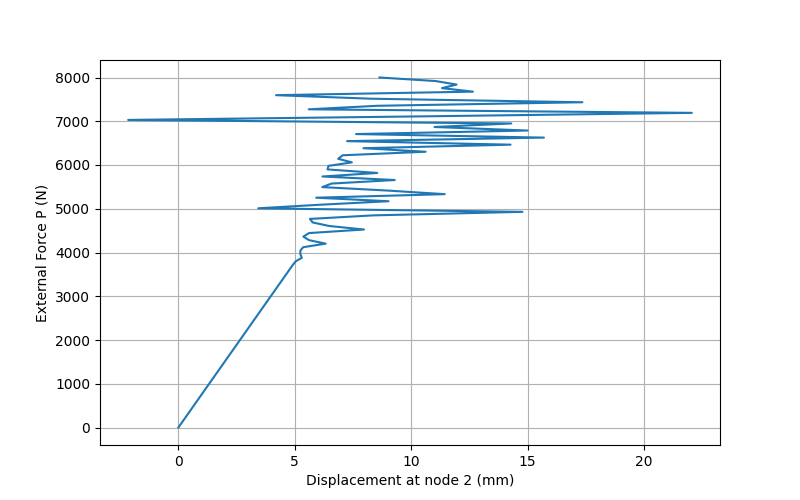
\includegraphics[width=\linewidth]{media/apotyxia1.png}
        \caption{Διάγραμμα δύναμης προς μετατόπιση.}
    \end{subfigure}
    \hfill
    \begin{subfigure}{0.3\linewidth}
        \centering
        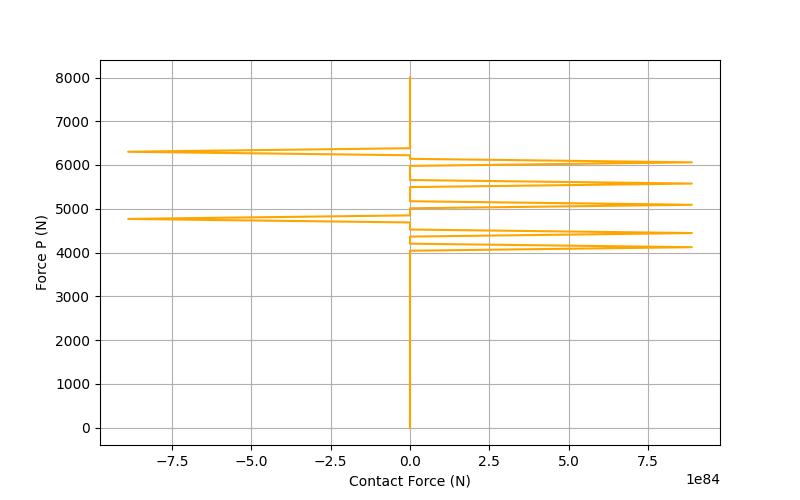
\includegraphics[width= \linewidth]{media/apotyxia22.png}
        \caption{Διάγραμμα δύναμης προς δύναμη αντίδρασης.}
    \end{subfigure}
    \hfill
    \begin{subfigure}{0.3\linewidth}
        \centering
        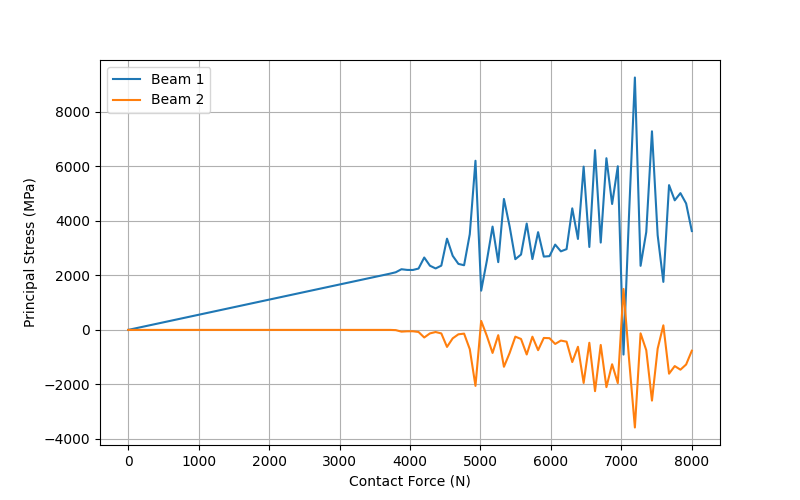
\includegraphics[width=\linewidth]{media/apotyxia3.png}
        \caption{Διάγραμμα τάσης προς εξωτερική δύναμη.}
    \end{subfigure}
    \caption{Αποτυχημένη επίλυση με πολύ μεγάλη σταθερά ποινής, ίση με 1E100.}
    \label{fig:astox}
\end{figure}

Τα αποτελέσματα που προκύπτουν πραγματικά, συμφωνούν με τη θεωρία. Η μετατόπιση όπως φαίνεται αυξάνεται υπό σταθερή κλίση έως το σημείο επαφής. Έπειτα αυξάνεται με πολύ μεγαλύτερη κλίση.

\begin{figure}[H]
    \centering
    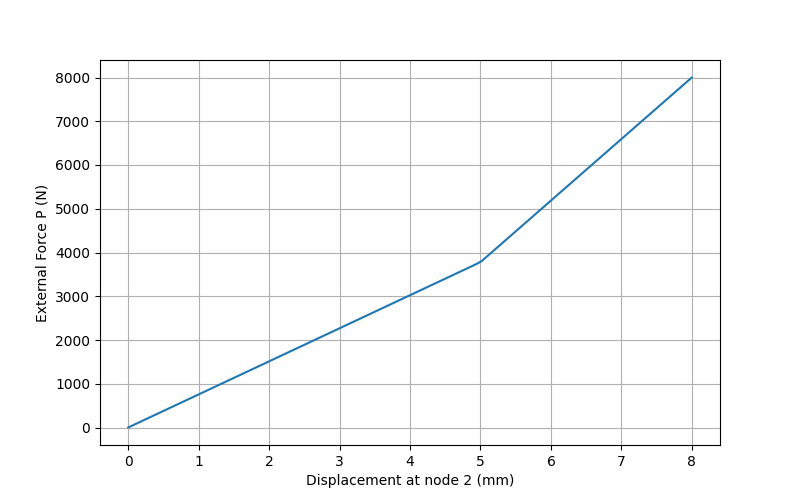
\includegraphics[width=0.8\linewidth]{media/Fu.png}
    \caption{Διάγραμμα δύναμης προς μετατόπιση του κόμβου 2, δηλαδή του κόμβου της επαφής.}
    \label{fig:a1}
\end{figure}


\begin{figure}[H]
    \centering
    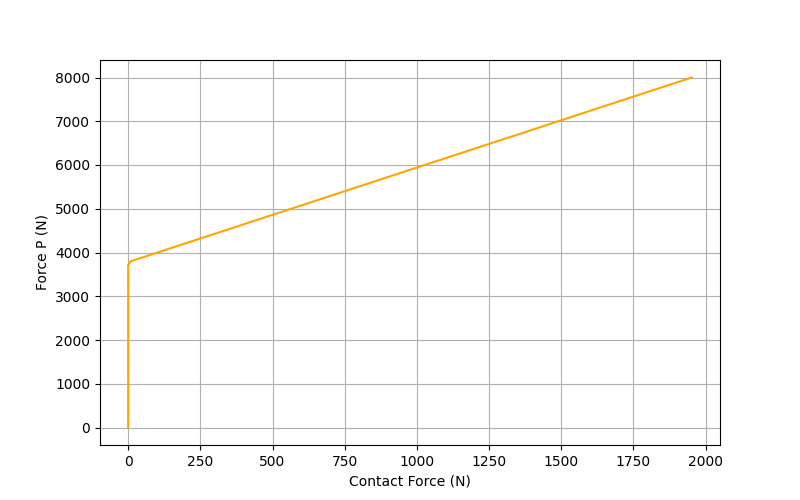
\includegraphics[width=0.8\linewidth]{media/FR.png}
    \caption{Διάγραμμα δύναμης προς αντίδραση επαφής.}
    \label{fig:a2}
\end{figure}


\begin{figure}[H]
    \centering
    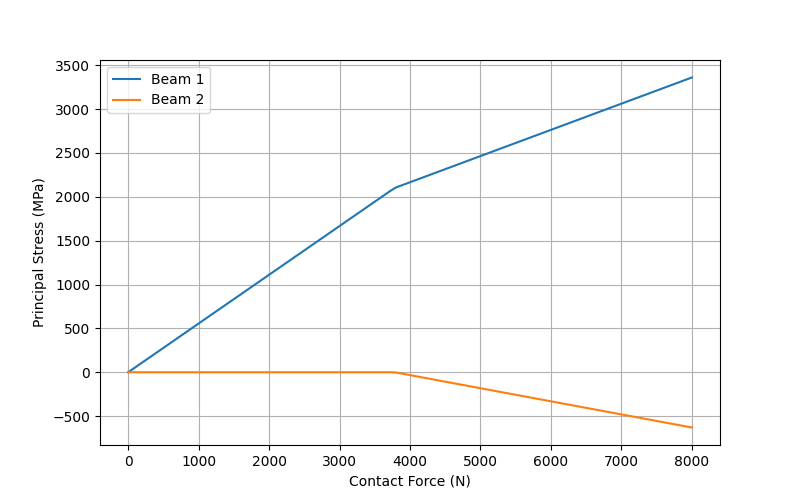
\includegraphics[width=0.8\linewidth]{media/sF.png}
    \caption{Διάγραμμα τάσης προς την εξωτερική δύναμη στον κόμβο 2.}
    \label{fig:a3}
\end{figure}



\subsection{Μέρος Β'}
Όσο αναφορά το δεύτερο μέρος, τα μοντέλα με πυκνό πλέγμα αποδείχθηκαν πολύ ικανοποιητικά καθώς έρχονται σε ταύτιση με τα θεωρητικά αποτελέσματα. Προφανώς, τα μοντέλα με αδρό πλέγμα δεν απέδωσαν καλά. Όσο πιο μακριά από το σημείο επαφής υπολογίζεται τιμή τόσο πιο κοντά στη θεωρητική της βρίσκεται. Επίσης, τα μοντέλα με αδρό πλέγμα αποδείχθηκαν εντελώς ανίκανα να υπολογίσουν τη συνάρτηση της πίεσης. Σχετικά με τη δύναμη, όλα τα μοντέλα έρχονται σε ταύτιση με την αναλυτική λύση.


\begin{figure}[H]
    \centering
    \begin{subfigure}{0.49\linewidth}
        \centering
        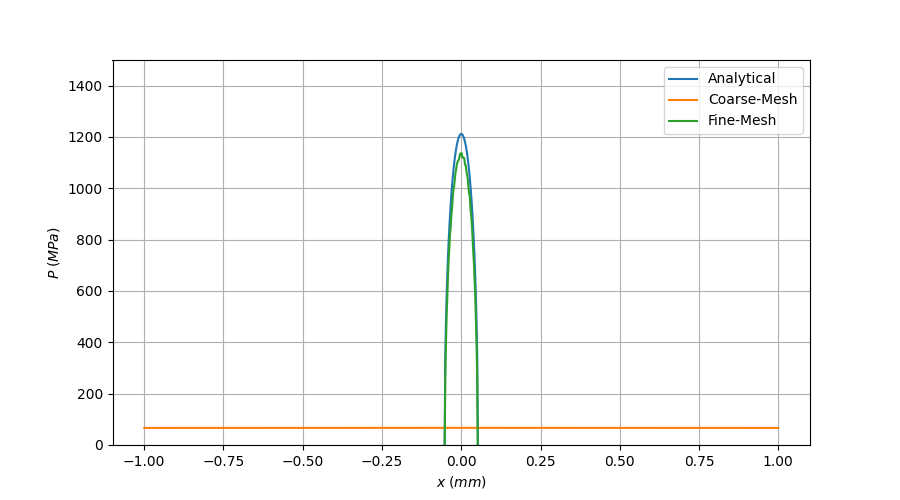
\includegraphics[width=\linewidth]{media/plin.png}
        \caption{Πρόβλημα γραμμικής επαφής.}
    \end{subfigure}
    \hfill
    \begin{subfigure}{0.49\linewidth}
        \centering
        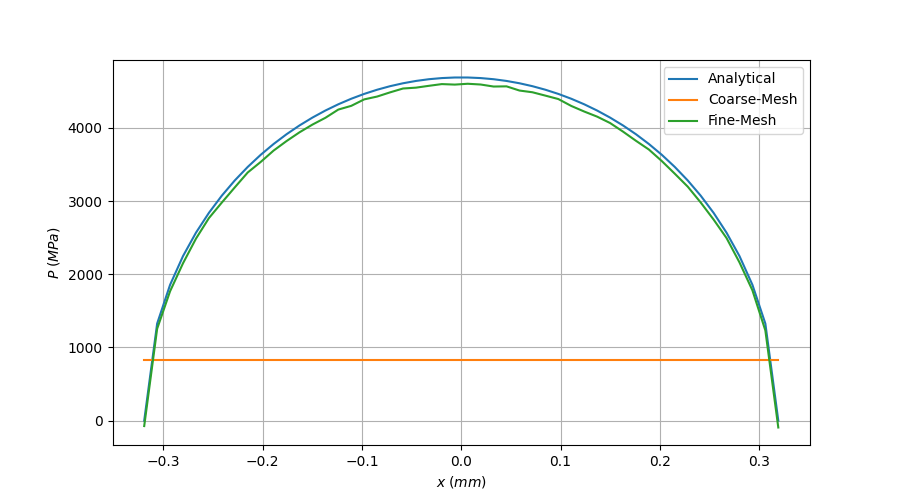
\includegraphics[width=\linewidth]{media/pp.png}
        \caption{Πρόβλημα σημειακής επαφής.}
    \end{subfigure}
    \caption{Πίεση επαφής.}
    \label{fig:b1}
\end{figure}

\begin{figure}[H]
    \centering
    \begin{subfigure}{0.49\linewidth}
        \centering
        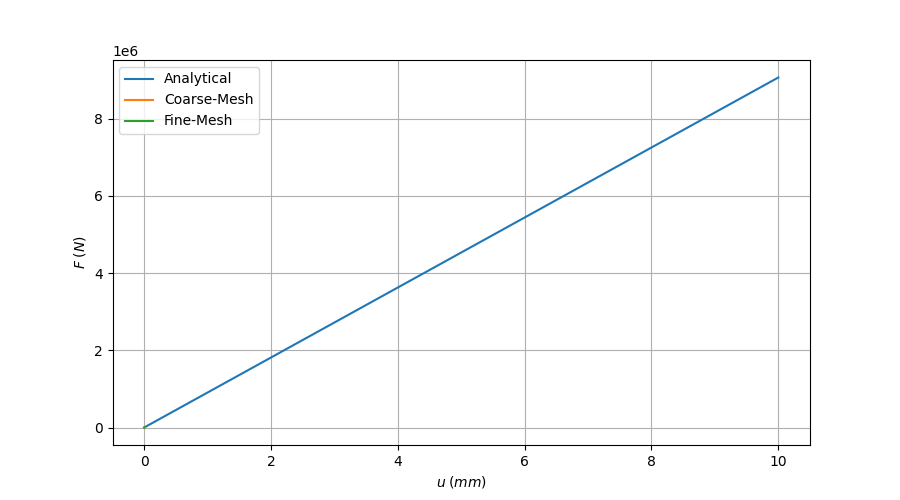
\includegraphics[width=\linewidth]{media/flin.png}
        \caption{Πρόβλημα γραμμικής επαφής.}
    \end{subfigure}
    \hfill
    \begin{subfigure}{0.49\linewidth}
        \centering
        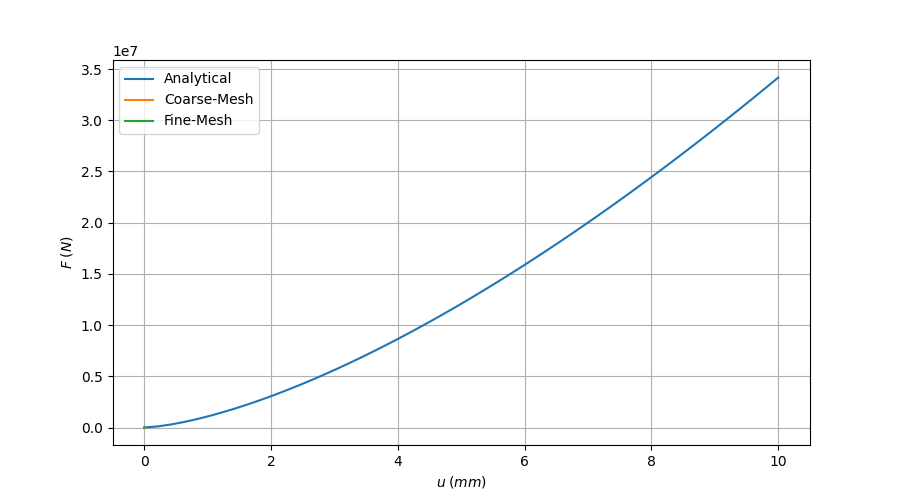
\includegraphics[width=\linewidth]{media/fp.png}
        \caption{Πρόβλημα σημειακής επαφής.}
    \end{subfigure}
    \caption{Σχέση δύναμης προς μετατόπιση.}
    \label{fig:b2}
\end{figure}



\begin{figure}[H]
    \centering
    \begin{subfigure}{0.32\linewidth}
        \centering
        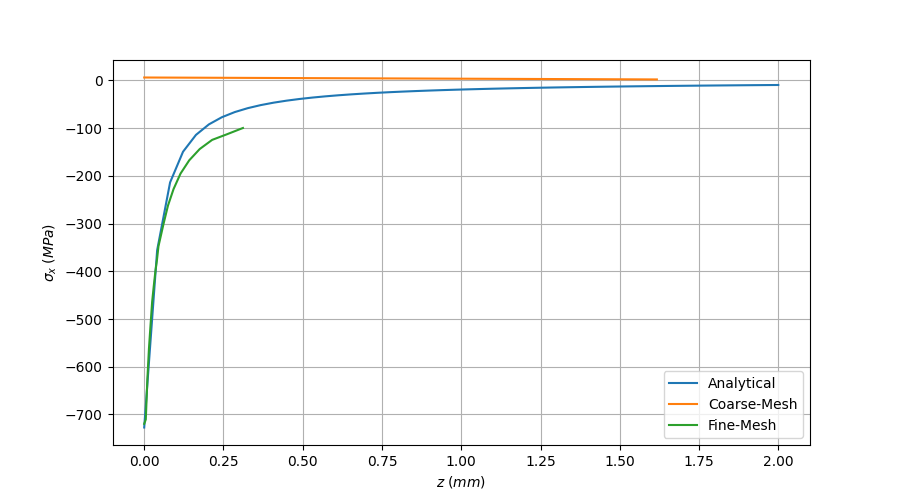
\includegraphics[width=\linewidth]{media/sxlin.png}
        \caption{$\sigma_x$}
    \end{subfigure}
    \hfill
    \begin{subfigure}{0.32\linewidth}
        \centering
        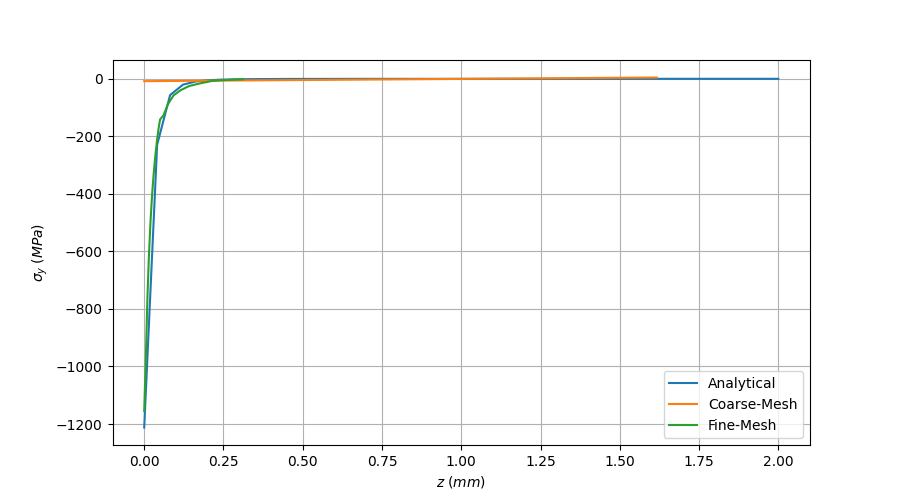
\includegraphics[width= \linewidth]{media/sylin.png}
        \caption{$\sigma_y$}
    \end{subfigure}
    \hfill
    \begin{subfigure}{0.32\linewidth}
        \centering
        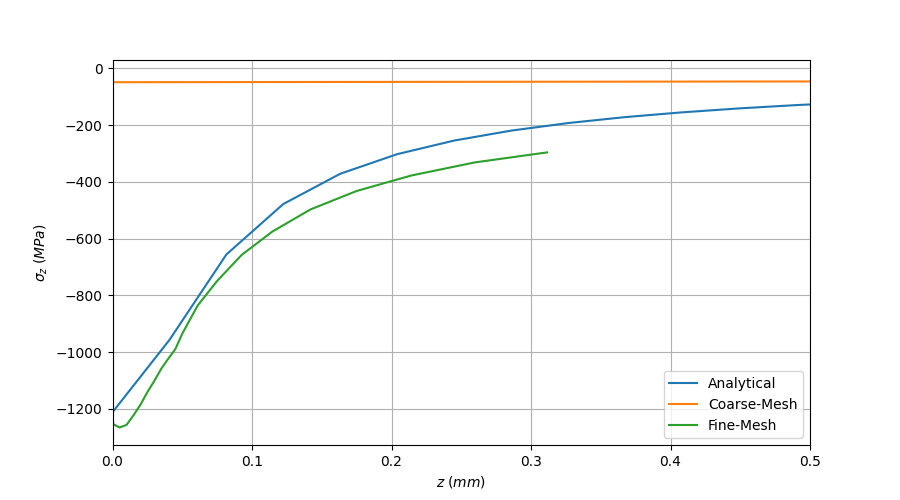
\includegraphics[width=\linewidth]{media/szlin.png}
        \caption{$\sigma_z$}
    \end{subfigure}
    \caption{Κύριες τάσεις επαφής για το πρόβλημα γραμμικής επαφής.}
    \label{fig:b3}
\end{figure}


\begin{figure}[H]
    \centering
    \begin{subfigure}{0.49\linewidth}
        \centering
        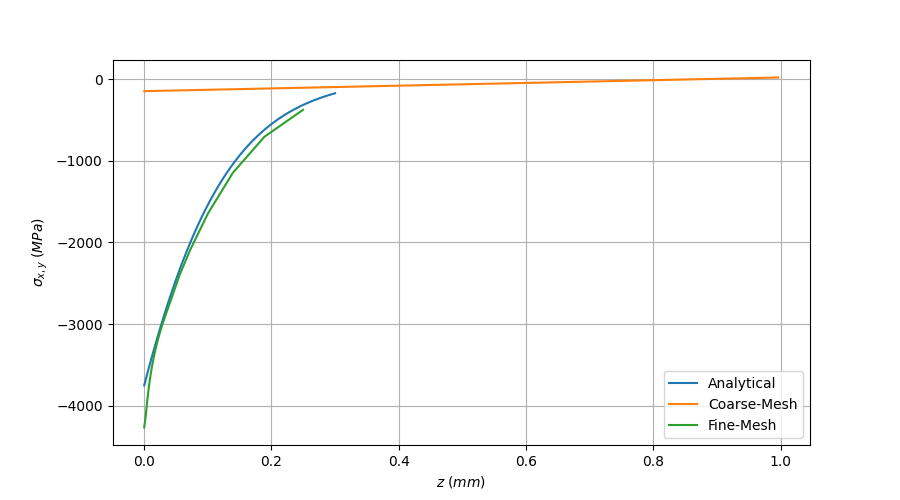
\includegraphics[width=\linewidth]{media/sxp.png}
        \caption{$\sigma_{x,y}$}
    \end{subfigure}
    \hfill
    \begin{subfigure}{0.49\linewidth}
        \centering
        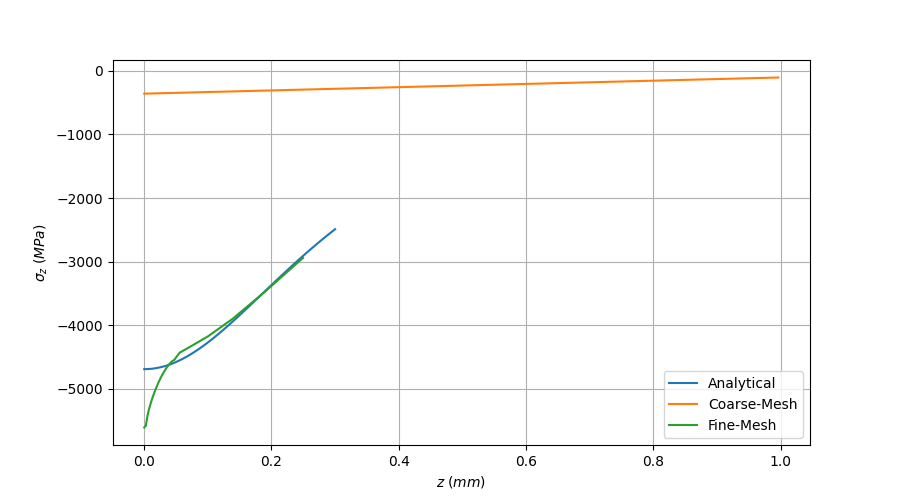
\includegraphics[width=\linewidth]{media/szp.png}
        \caption{$\sigma_{z}$}
    \end{subfigure}
    \caption{Κύριες τάσεις επαφής για το πρόβλημα σημειακής επαφής.}
    \label{fig:b4}
\end{figure}







\end{document}